\documentclass[12pt]{article}
%	options include 12pt or 11pt or 10pt
%	classes include article, report, book, letter, thesis

% \usepackage[margin=0.75in]{geometry}
\usepackage[margin=1in]{geometry}
\setlength{\parindent}{0pt}

\usepackage{hyperref}

%for writing of code in blocks like
%\begin{lstlisting}
%   .......
%\end{lstlisting}
\usepackage{listings}
\usepackage{color}
\usepackage{enumitem}
\usepackage{graphicx}
\usepackage{url}

\definecolor{dkgreen}{rgb}{0,0.6,0}
\definecolor{gray}{rgb}{0.5,0.5,0.5}
\definecolor{mauve}{rgb}{0.58,0,0.82}

\lstset{frame=tb,
  language=C++,
  aboveskip=3mm,
  belowskip=3mm,
  showstringspaces=false,
  columns=flexible,
  basicstyle={\small\ttfamily},
  numbers=none,
  numberstyle=\tiny\color{gray},
  keywordstyle=\color{blue},
  commentstyle=\color{dkgreen},
  stringstyle=\color{mauve},
  breaklines=true,
  breakatwhitespace=true,
  tabsize=3
}
%%%%%%%%%%%%%%%%%%%%%%

\title{Life of a Particle : Assignment 1}
\author{Claire David}
\date{Due Date : DD/MM/2019}

\begin{document}
\vspace{-2ex}
\maketitle

\textbf{How to submit}
\newline
This assignment should be submitted by replying to the email sent out requesting its submission.\\
You should include a single PDF file that has any verbal description of the answers to the questions, along with description of what computer code files go with which question.\\
Please bundle this all into a single tarball and submit this one tarball file.\\
Naming convention: {\tt{lifefofparticle\_part2\_assignment1\_YOURNAME.tar}}

\section*{Interpreting test beam data}

The following plot comes from real data taken at the DESY II testbeam facility in Hamburg, Germany. 


\begin{figure}[h]
    \centering
    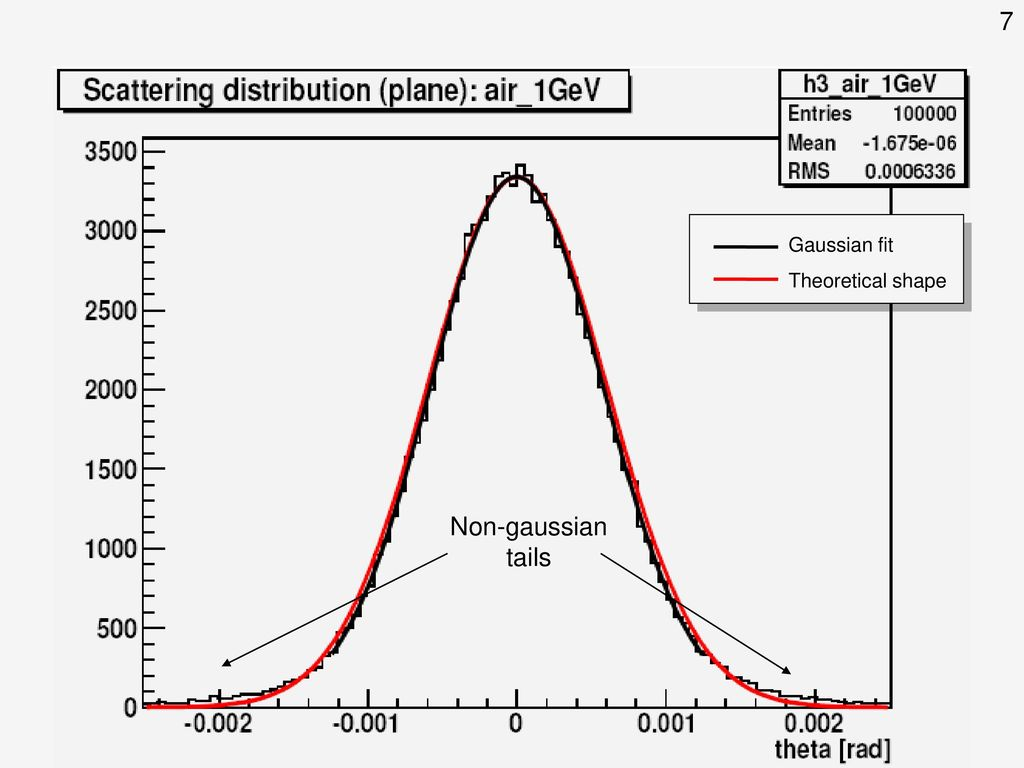
\includegraphics[width=0.6\textwidth]{electron_scattering_DESY_2006.jpg}
%     \caption{}
%     \label{fig:mesh1}
\end{figure}

A test beam telescope consists of aligned sensitive plates perpendicular to the beam direction $\vec{e}_z$, which record the position along the $\vec{e}_x$ and $\vec{e}_y$ directions.\\
The ``EUDET''-type telescope have six of such plates. Between the third and fourth ones, a sample of material or device to test, called testbeam target, is inserted.\\
By measuring the tracks formed by the hits on the first three plates and the tracks after scattering of the electron on the 
target on the last three sensors, it is possible to compute a scattering angle. This physical quantity is linked to a characteristic of the tested material: 
the radiation length $X_0$ or material budget. $X_0$ corresponds to the distance over which a high-energy electron loses all but $1/e$ of its energy by Bremsstrahlung.\\

If you are curious, you can read more about the testbeam facilities and the telescopes here:\\
\hspace{10ex} \href{http://particle-physics.desy.de}{http://particle-physics.desy.de}\\[1ex]
\hspace{10ex} \href{https://telescopes.desy.de}{https://telescopes.desy.de}\\[1ex]

Note: the distribution above has no target material, only air. This setup serves as calibration.

We saw in class that the deflection of the passing particles on the last detector layer can be approximated with a Gaussian distribution:

\begin{figure}[h]
    \centering
    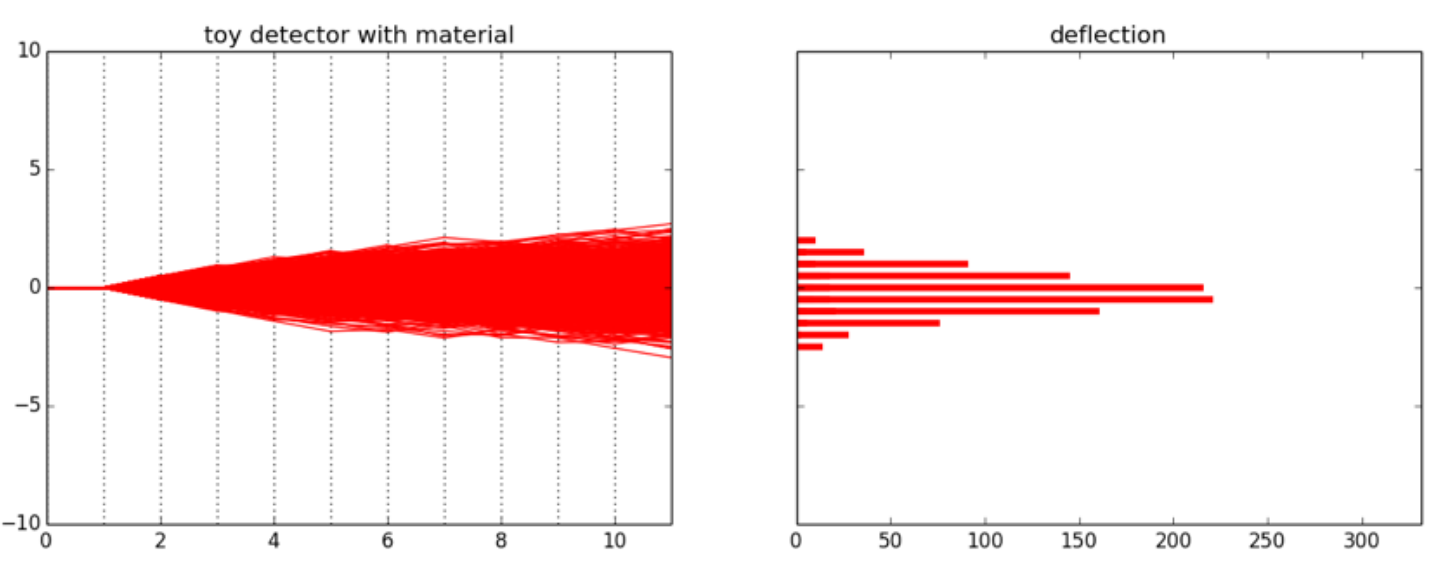
\includegraphics[width=0.75\textwidth]{toy_det_deflection.png}
%     \caption{}
%     \label{fig:mesh1}
\end{figure}

A) Adapt the program to reproduce the DESY setup and generate overlaid tracks. For which number of track is a Gaussian distribution clear?\\[1ex]

B) Get the file {\tt{testbeam\_data.root}} and draw the histogram. What are the parameters of this Gaussian?\\[1ex]

C) Re-run the toy detector incorporating these parameters to model the data. How is the agreement at the center of the plane? And in the edge/tail of the distribution?\\[1ex]

D) Add in the program a separate scattering process (that you should guess) that could explain and model these non-Gaussian tails.\\[1ex]

\vspace{1ex}
\textit{BONUS:}\\
We now insert in the telescope a piece of unknown material, 3 mm thick (along the beam direction $\vec{e}_z$). The distribution of the deflection angle $\theta$ is stored in the file {\tt{target\_X\_distrib.root}}\\[1ex]
Using the Moliere formula, compute the radiation length of this unknown material. By comparing with tables in the literature, which material is it?\\
{\color{red}\textbf{TODO provide files histogram of testbeam data and BONUS files and numbers}}

\end{document}